\section{Introduction}
\subsection{Problem Description}
The main goal of the activity described in this report is the following: realizing a network implementing a \textbf{perceptron} with a \textbf{sigmoid activation function}.\\
Before describing the whole design and implementation process a very little introduction about the architecture must be done.\\

\begin{figure}[h]
	\centering
	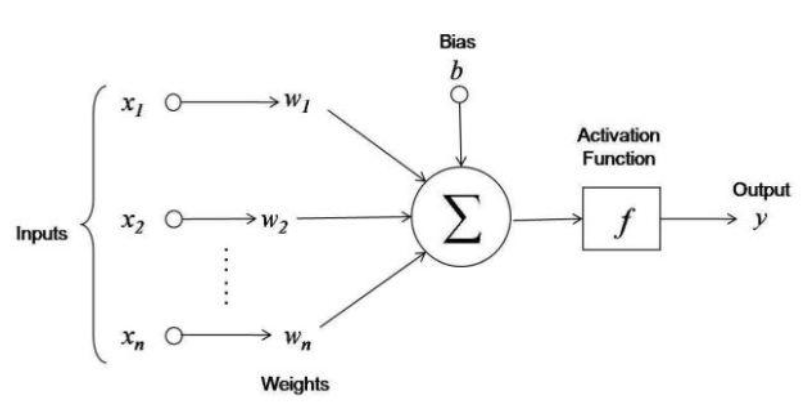
\includegraphics[width=\textwidth]{img/perceptron.png}
	\caption{Perceptron Architecture}
\end{figure}

A \textbf{Perceptron} is a \textit{binary classifier that maps his inputs to a specific output y = f(z), where f() is the \textbf{activation function} of the perceptron.} The inputs are real numbers and the input z of the activation function is obtained as:\\
\begin{equation}
	z = b + \sum_{i = 0}^{N_{L}-1}w_{i}x_{i}
\end{equation}

Every input $x_{i}$, every weight $w_{i}$ and the bias $b$ are real numbers in the range of $[-1, 1]$. \\
The \textbf{activation function}, in our case, will be a \textbf{sigmoid function}, described as follows:
\begin{figure}[h]
	\centering
	\caption{Sigmoid Function Plot}
	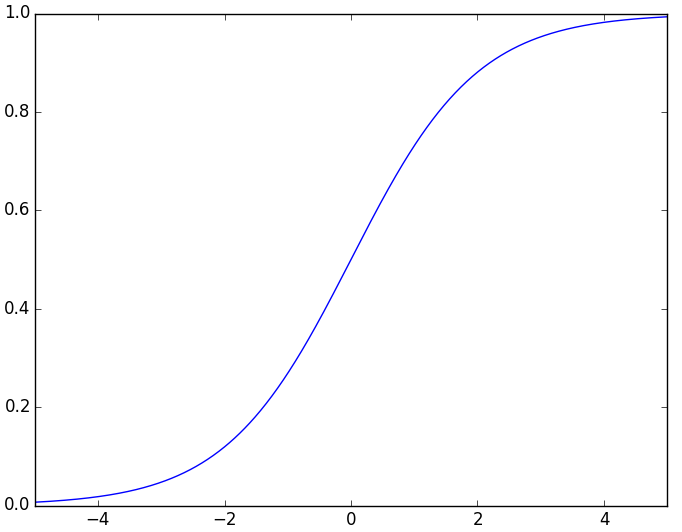
\includegraphics[width=8cm]{img/sigmoid.png}
\end{figure}
\begin{equation}
	y = \dfrac{1}{1+e^{-z}}
\end{equation}
Where $z$ is the result of the equation (1.1).
\subsection{Applications}
A single perceptron is the building block of \textit{artificial neural networks}, in which different layers of perceptrons are connected. The output of the neural network is a real number and could be use to classify \textit{complex objects}: patterns, human faces, handwritings, medical diagnosis, e-mail spams.\\
\begin{figure}[H]
	\centering
	\caption{Neural network example}
	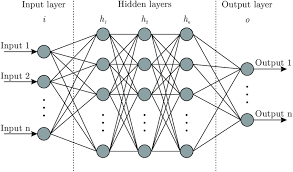
\includegraphics[width=8cm]{img/neural_network.png}
\end{figure}
In the image above there is a simple schema of a neural network, in which the circles represent the perceptrons.
\subsection{Possible Architectures}

The main architecture will be made up by three main logical parts, from an higher-lever point of view:
\begin{itemize}
	\item \textbf{Multiplication Circuit}: implementation of the multiplication operation between each input $x_{i}$ and each weight $w_{i}$.
	\item \textbf{Adder Circuit}: implementation of the addition between the results of the former phase and the bias $b$.
	\item \textbf{Activation Function Circuit}: implementation of the computation of the sigmoid function.
\end{itemize}

In the next chapter the architecture will be documented with more precision.
Different project choices could be made for each logical part of the architecture:

\begin{itemize}
	\item{\textbf{Multiplication Circuit}}: could be implemented through a \textbf{ROM-based solution} in which every possible result is stored and the two inputs represent the addresses for getting the result. This solution is good only with a very low number of bits, which is not our case: in fact the the ROM will be composed by $2^{(n_{w_{i}} + n_{b_{i}})}$ memory cells. In order to implement the multiplication circuit will be implemented through a  \textbf{Paraller Multiplier}.
	\item{\textbf{Adder Circuit}}: different choice could be made to implement the adder circuit. Starting from the simplest to the more complex solution we can exploit the \textbf{Serial Adder}, the \textbf{Parallel Adder} or the \textbf{Parallel Adder with Pipeline }. The first one needs less logic but requires $n$ clock cycles for computing an $n$ bits result. The second solution improves the first one by computing one result in \textbf{one clock cycle}, on the other hand it could add some problems due to long logic chains between two register. The third solution is the best from the perspective of the number of clock cycles required and the \textbf{critical path}, in fact by adding some registers in between the computation of the bits will reduce the logic chains. 
	\item{\textbf{Activation Function Circuit}}: As seen during the laboratory class, this part will be implemented by exploiting a Look-Up-Table. In order to do so, could be necessary a \textbf{truncation} of the result of the former computation in order to limit the size of the LUT. With $12$ bits are necessary $2^{12} = 4096$ entries, which could be even reduced by performing some optimization by exploiting the sigmoid function symmetry.
\end{itemize} 
